\section{Sistemas embebidos}
	Un sistema embebido es una combinación de hardware y software integrado para realizar una función particular. Son controlados por un microcontrolador o microprocesador incrustada en ellos, lo que implica que se encuentra dentro del sistema general, oculto a la vista, formando una parte integral de un conjunto mayor. \cite{vahid1999} \\
	
	Los sistemas embebidos tienen varias características comunes, como: ejecutar sólo un programa repetidamente, tiene un diseño optimizado para reducir costo y espacio, contienen sólo los recursos de hardware suficientes para cumplir con  los  requerimientos  de  funcionalidad  de  la  aplicación. \cite{kamal2008} \\
	
%	\subsection{Arquitectura de los sistemas embebidos}
	Un sistema embebido cuenta con varios componentes que permiten que cumpla con las características mencionadas anteriormente. En la figura \ref{fig:MarcoArquiSE} se muestran de forma general la arquitectura de un sistema embebido con todas las partes que lo componen, las cuales se describen a continuación. \cite{nadalEmbebidos} \cite{heath2005}
	
	\begin{enumerate}
		\item \textbf{Hardware.} Es el recurso fundamental de cualquier sistema embebido y la elección de éste depende de las especificaciones del diseñador.
		
		\item \textbf{Unidad de Procesamiento (CPU).} Es el componente encargado de realizar las operaciones de cálculo principales del sistema. Ejecuta código para realizar una determinada tarea y dirige el funcionamiento de los demás elementos que le rodean. Se prefiere un microcontrolador para construir aplicaciones pequeñas con cálculos precisos. Un Sistema en Chip (SoC) incluye una CPU, dispositivos periféricos (temporizadores, contadores), interfaces de comunicación (I2C, SPI, UART) y circuitos de administración de energía en un solo circuito integrado.
		
		\item \textbf{Interfaces de entrada.} Establecen la comunicación entre la unidad de procesamiento y el proceso, filtrando, adaptando y codificando de forma comprensible las señales procedentes de los dispositivos de entrada. Algunos de los ejemplos de dispositivos de entrada son: ADC, señales de sensores, módulos de cámara digital, etc. Es importante recalcar que algunos de los dispositivos de entrada se comunican con la unidad de procesamiento haciendo uso de alguna interfaz como SPI, I2C o UART.
		
		\item \textbf{Dispositivos de entrada.} Los dispositivos de entrada toman valores del mundo exterior. Estos dispositivos pueden ser sensores, interruptores, fotodiodos, entre otros.
	
		\item \textbf{Interfaces de salida.} Después de haber obtenido datos mediante los dispositivos de entrada, la unidad de procesamiento trabaja con esos datos y envía el resultado mediante las interfaces de salida. En estas interfaces establecen la comunicación entre el sistema embebido y el usuario o dispositivo final. Algunos ejemplos de dispositivos de salida son: módulos WiFi, LCD, LED, motores, entre otros. 
		
		\item \textbf{Memoria.} La memoria esencialmente realiza dos funciones principales dentro de un sistema embebido, una de ellas es proporcionar almacenamiento para el software que se ejecutará y proporcionar almacenamiento para datos como variables de programa y resultados intermedios, información de estado y cualquier otro dato que pueda crearse durante la operación.
		
		\item \textbf{Software.} Los componentes de software dentro de un sistema embebido son esenciales para el control del sistema embebido, definiendo qué hace y qué tan bien lo hace.
	\end{enumerate}
	
\clearpage	
	\begin{figure}[htbp!]
		\centering
		\fbox{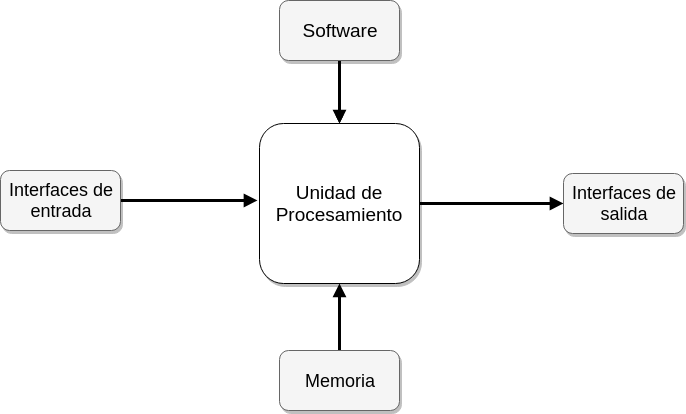
\includegraphics[width=0.8\textwidth]{MarcoTeorico/imagenes/arquitecturaSE.png}}
		\caption{Arquitectura general de un sistema embebido.}
		\label{fig:MarcoArquiSE}
	\end{figure}
%	\TOCHK{Agregar imagen y descripción de su arquitectura}
%	\subsection{Aplicaciones}

	Los sistemas embebidos tienen una gran cantidad de aplicaciones dentro de casas inteligentes, oficinas, transporte, cuidado de la salud, industrias, entre otros. \\
	
	En el caso del cuidado de la salud (healthcare), los sistemas embebidos se utilizan para monitorear los signos vitales, para amplificar sonidos en estetoscopios electrónicos y para casi cualquier sistema de imágenes, además de una gran variedad de equipo biomédico. Estas aplicaciones permiten a los médicos monitorear de forma remota la salud de sus pacientes y tomar decisiones de diagnóstico y tratamiento a través de la telemedicina y otros sistemas remotos. \cite{delkinEmbSys} \\
	
	El Internet de las cosas (IoT) es un concepto y un paradigma que considera la presencia generalizada en el entorno de una variedad de cosas/objetos que contienen tecnología integrada para comunicarse a través de conexiones alámbricas e inalámbricas con el fin de interactuar entre sí y cooperar con otras cosas/objetos para crear nuevas aplicaciones/servicios y alcanzar objetivos comunes. \cite{vermesanIoT}
	
	De acuerdo a lo anterior podría decirse que el Internet de las cosas y los sistemas embebidos son conceptos que no pueden tratarse por separado tan fácilmente.

%\clearpage
\pagebreak